\documentclass[a4paper,12pt,titlepage]{article}
\usepackage{amsmath} 
\usepackage{amssymb}
\usepackage[nottoc]{tocbibind}
\usepackage{mathrsfs}
\usepackage{float}
\usepackage{indentfirst}
\author{\textit{Jiang Yicheng}\\\textit{515370910224}}
\title{\textbf{VE203\\
		Assignment 7}}
\date{\today}
\usepackage{dsfont}
\usepackage[top=1in, bottom=1in, left= 1in, right=1in]{geometry}
\usepackage{fancyhdr,lastpage}
	\pagestyle{fancy}
	\fancyhf{}
\cfoot{Page \thepage\ of \pageref{LastPage}}
\usepackage{multirow}
\usepackage{gauss}
\usepackage[colorlinks=true,linkcolor=black]{hyperref}
\usepackage[linesnumbered,ruled,longend]{algorithm2e}
\SetKwInOut{Input}{Input}
\SetKwInOut{Output}{Output}
\newcommand{\To}{\KwTo}
\newcommand{\Ret}{\KwRet}
\SetKwProg{Fn}{Function}{\string:}{end}
\SetKwFunction{mc}{MC}
\newcommand{\udots}{\mathinner{\mskip1mu\raise1pt\vbox{\kern7pt\hbox{.}}\mskip2mu\raise4pt\hbox{.}\mskip2mu\raise7pt\hbox{.}\mskip1mu}}
\SetKwFunction{pow}{PowMod}
\usepackage{graphicx}
\usepackage{extarrows}
\begin{document}

\maketitle

\section*{Exercise 7.1} 
\subsection*{i)}
\begin{figure}[H]
	\centering
	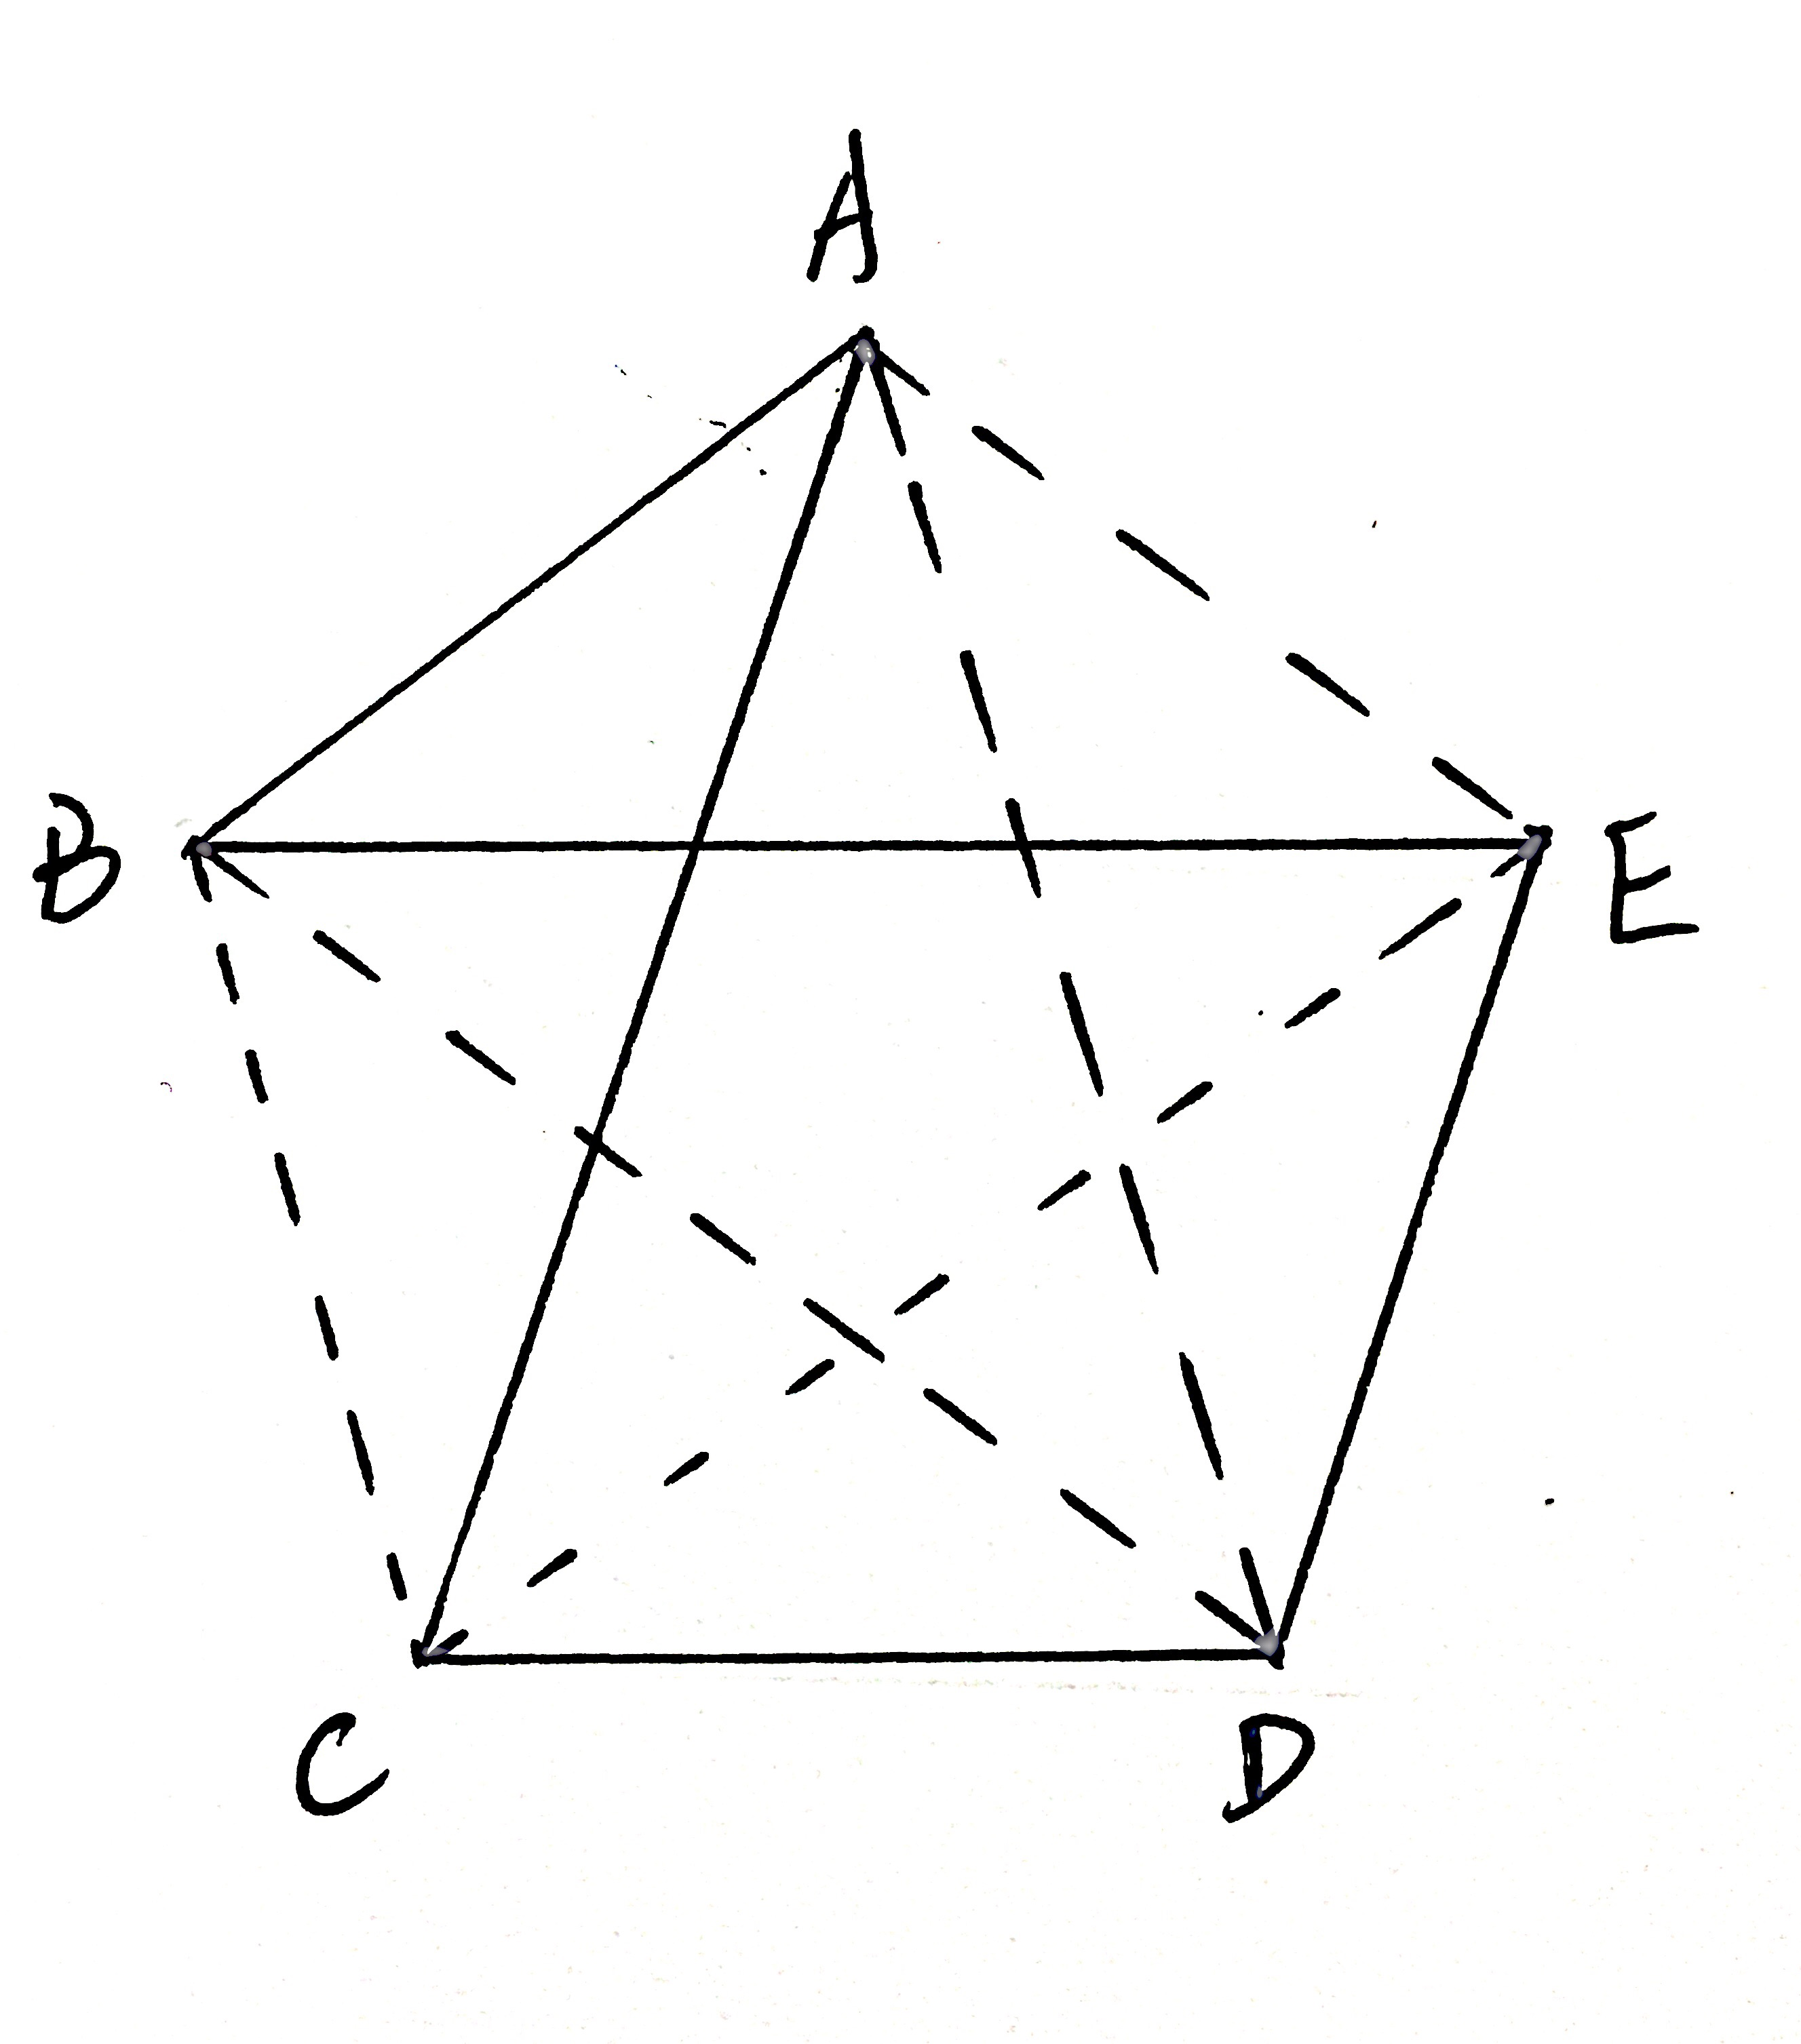
\includegraphics[scale=0.1]{1.jpg}
\end{figure}
We use five different points to denote five people in the party, and connect two points with full line if two people are friends and connect two points with dash line.
 
As the figure shows, there doesn't exist a triangle whose three sides are all full line or dash line, which means that in these five people there are no three people are enermies each other or firends each other. 

Hence, $R(3,3)>5$.

\subsection*{ii)}
Consider one member of the party, A. The nine other members of the party
are either friends or enemies of A. By the generalized pigeonhole principle, at least five of them are either friends or enemies of A. 

Suppose that B, C, D, E, F are friends of A.  If any two of these five people are friends, then they together with A are a group of three mutual friends. If none of B, C, D, E, F are friends, then any four of them form a group of four mutual enemies.

If B, C, D, E, F are a group of five enemies of A, the proof proceeds in a
similar manner.

So in a group of 10 people there are either three mutual friends or four mutual enemies, and there are either three mutual enemies or four mutual friends. Hence $R(4,3)\leqslant10$.

\subsection*{iii)}
Consider one member of the party, A. The nineteen other members of the party are either friends or enemies of A. By the generalized pigeonhole principle, at least ten of them are either friends or enemies of A. 

Suppose that B, C, D, E, F, G, H, I, J, K are friends of A. According to ii) there are either three mutual friends or four mutual enemies in these ten people. If B, C, D are three mutual friends, then together with A they are a group of four mutual friends; if there are four mutual enermies, that's just what we want. 

If B, C, D, E, F, G, H, I, J, K are a group of five enemies of A, the proof proceeds in a similar manner.

So in a group of 20 people there are either four mutual friends or four mutual enemies. Hence $R(4,4)\leqslant20$.

\subsection*{iv)}
For any $k\in\mathbb{N},k\leqslant n-1$, if they are all $k$ mutual enermies with each other, then there doesn't exist $n$ mutual enermies or two mutual friends. So $R(2,n)\geqslant n$. For any $n$ people, if there exist two people who are friends, that's what we want; if no two people are friends, then these $n$ people are mutual enermies. Hence, in any $n$ people at a party there are either 2 mutual friends or $n$ mutual enemies.

So $R(2,n)=n$.

\subsection*{v)}
In any $R(m-1,n)+R(m,n-1)$ people, consider one member of the party, A. The $R(m-1,n)+R(m,n-1)-1$ other members of the party are either friends or enemies of A. 

If there are at least $R(m-1,n)$ friends of A. In these people, there are either $m-1$ mutual friends or $n$ mutual enemies. If there are $m-1$ mutual friends, then together with A we find $m$ mutual friends; if there are $n$ mutual enemies, that's also what we want.

If there are no more than $R(m-1,n)-1$ friends of A, then there are at least $R(m,n-1)$ enermies of A. In these people, there are either $m$ mutual friends or $n-1$ mutual enemies. If there are $n-1$ mutual enermies, then together with A we find $n$ mutual friends; if there are $m$ mutual friends, that's also what we want.

So in a group of $R(m-1,n)+R(m,n-1)$ people there are either $m$ mutual friends or $n$ mutual enemies. Hence $R(m,n)\leqslant R(m-1,n)+R(m,n-1)$.

\subsection*{vi)}

In a party of size 9, if every person has five friends, then the total number of friends should be $5\times 9=45$. While since the relationship is symmetric which means that the total number should be an even number. And therefore there must be a person A who has at least 6 friends or at most 4 friends.   

If A has at least 6 friends. Since there are mutual 3 enermies or 3 friends in any 6 people, then together with A, there must be 3 mutual enermies or 4 mutual frineds. 

If A has at most 4 friends, then A should have at least 4 enermies B, C, D, E. If any two of these four people are enermies, then they together with A are a group of three mutual enermies. If none of B, C, D, E are eneimies, then they form a group of four mutual friends.

So in a group of 9 people there are either four mutual friends or three mutual enemies. Hence $R(4,3)\leqslant9$.

\subsection*{vii)}

\begin{figure}[H]
	\centering
	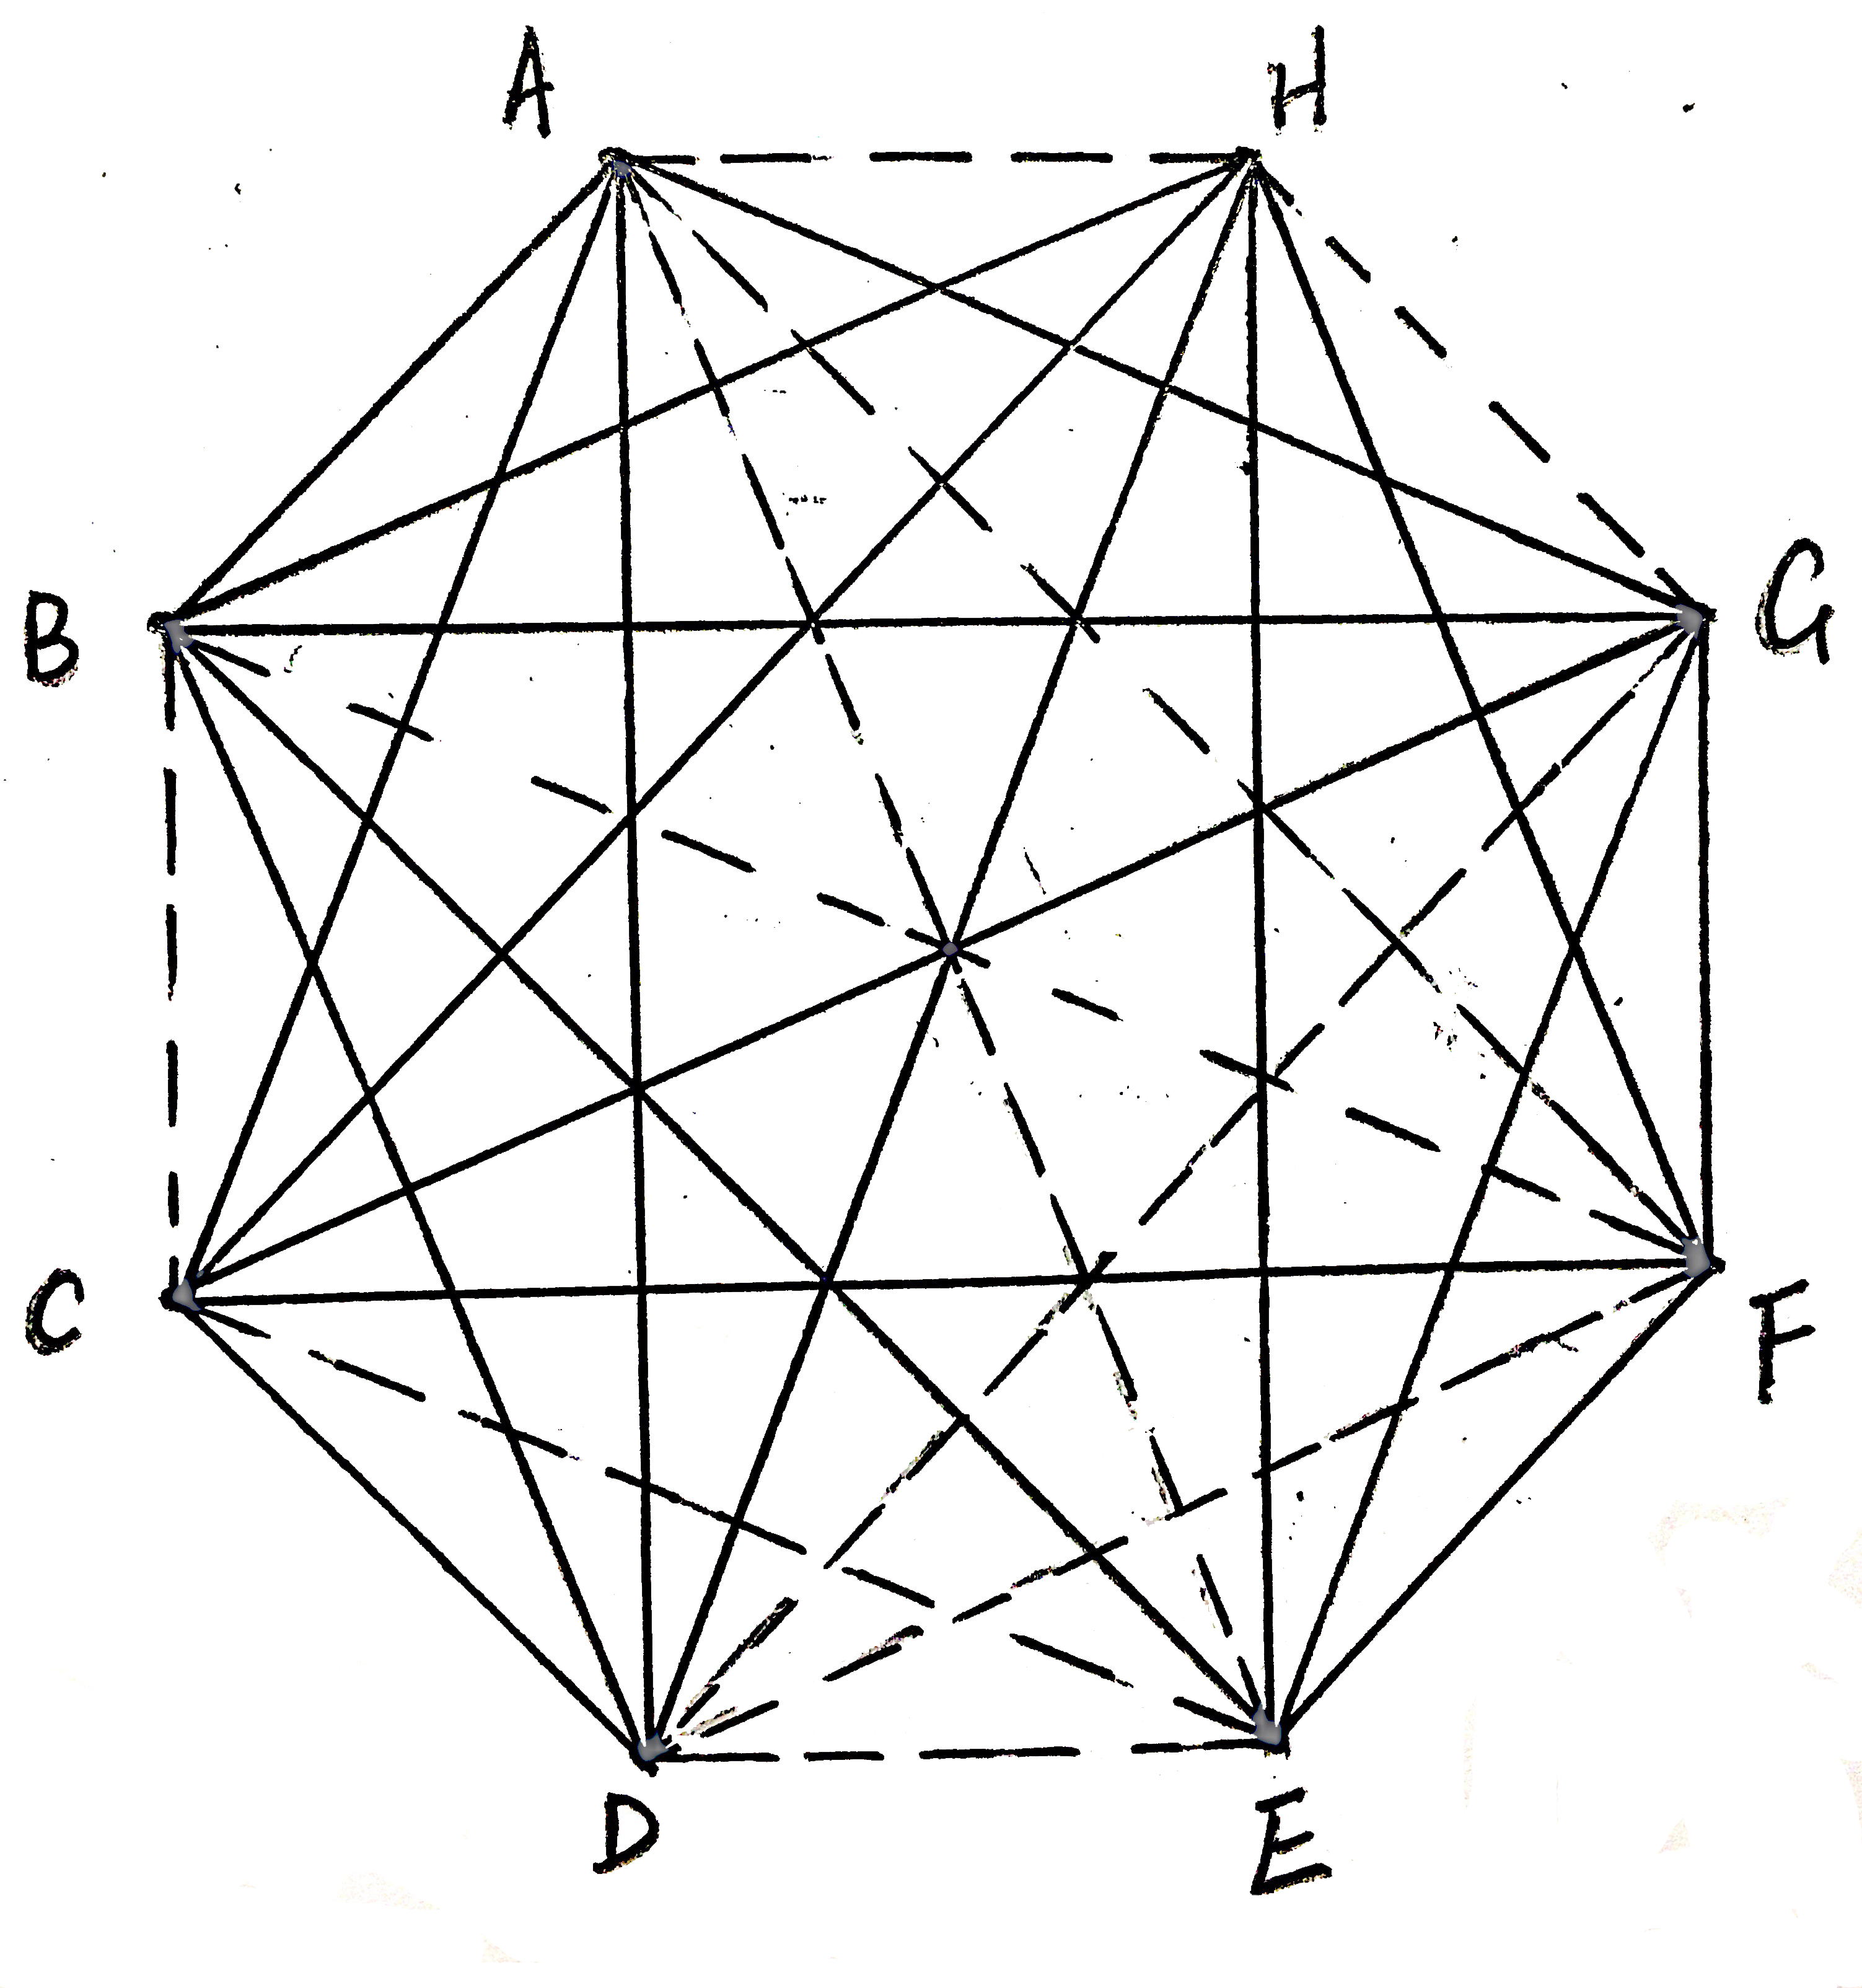
\includegraphics[width=10cm]{2.jpg}
\end{figure}

We use eight different points to denote eight people in the party, and connect two points with full line if two people are friends and connect two points with dash line.
 
As the figure shows, there doesn't exist a quadrilateral whose four sides and two diagonals are all full line and there doesn't exist a triangle whose three sides are dash line, which means that in these eight people there are no four people are friends each other and there are no three people are enermies each other. 

Hence $R(4,3)>8$. Then we can conclude that $R(4,3)=9$.

\section*{Exercise 7.2}
In a $n$ people party, if no two participants have the same number of friends, then all participants have different number of friends, so they have $0,1,2,\cdots,n-1$ friends respectively. However, the one have $n-1$ friends should be a friend of the one who has $0$ friend since there are $n$ people in total. That's impossible.

So there are two people at such a party that have the same number of friends.

\section*{Exercise 7.3}
We use induction to prove, $\forall n\in\mathbb{N}^*,1\leqslant k\leqslant n$, $\begin{pmatrix}
n\\
k
\end{pmatrix}\leqslant\dfrac{n^k}{2^{k-1}}$

\begin{enumerate}
\item When $k=1$, $\begin{pmatrix}
n\\
k
\end{pmatrix}=n\leqslant\dfrac{n^1}{2^{1-1}}$. So the statement holds when $k=1$.

\item Assume that when $k=m<n$, $\begin{pmatrix}
n\\
m
\end{pmatrix}\leqslant\dfrac{n^m}{2^{m-1}}$, then
\begin{align*}
\begin{pmatrix}
n\\
m+1
\end{pmatrix}-\dfrac{n^{m+1}}{2^{m}}&=\dfrac{n-m}{m+1}\dfrac{n!}{(n-m)!m!}-\dfrac{n^{m+1}}{2^{m}}\\
&\leqslant\dfrac{n-m}{m+1}\dfrac{n^m}{2^{m-1}}-\dfrac{n^{m+1}}{2^{m}}\\
&=\dfrac{n^m}{2^{m-1}}\dfrac{2n-2m-mn-n}{2(m+1)}\\
&\leqslant\dfrac{n^m}{2^{m-1}}\dfrac{-2m}{2(m+1)}\\
&<0
\end{align*}
So $\begin{pmatrix}
n\\
m+1
\end{pmatrix}<\dfrac{n^{m+1}}{2^{m}}$ which shows that the statement also holds for $k=m+1$
\end{enumerate}

To sum up, $\forall n\in\mathbb{N}^*, \forall k\in[1,n]\cap\mathbb{N}$, $\begin{pmatrix}
n\\
k
\end{pmatrix}\leqslant\dfrac{n^k}{2^{k-1}}$.


\section*{Exercise 7.4}
For any events $A,B$ and a probability function $P$ 
$$P[A\cup B]\leqslant 1,P[A\cup B]=P[A]+P[B]-P[A\cap B]$$
so
$$P[A\cap B]=P[A]+P[B]-P[A\cup B]\geqslant P[A]+P[B]-1$$

\section*{Exercise 7.5}
We prove by induction
\begin{enumerate}
\item When $n=2$, it's just $P[A\cup B]=P[A]+P[B]-P[A\cap B]$

\item Assume that $\forall n\leqslant k$, we have 
\begin{align*}
P[A_1\cup A_2\cup\cdots\cup A_n]=&\sum\limits_{1\leqslant i\leqslant n}P(A_i)-\sum\limits_{1\leqslant i<j\leqslant n}P[A_i\cap A_j]+\sum\limits_{1\leqslant i<j<k\leqslant n}P[A_i\cap A_j\cap A_k]\\
&-\cdots+(-1)^{n+1}P[A_1\cap A_2\cap\cdots\cap A_n]
\end{align*}
Then 
\begin{align*}
&P[A_1\cup A_2\cup\cdots\cup A_k\cup A_{k+1}]\xlongequal[B_i:=A_i(i<k)]{B_k:=A_k\cup A_{k+1}}P[B_1\cup B_2\cup\cdots\cup B_k]\\
=&\sum\limits_{1\leqslant i\leqslant k}P(B_i)-\sum\limits_{1\leqslant i<j\leqslant k}P[B_i\cap B_j]+\sum\limits_{1\leqslant i<j<l\leqslant k}P[B_i\cap B_j\cap B_l]\\
&-\cdots+(-1)^{k+1}P[B_1\cap B_2\cap\cdots\cap B_k]\\
=&\sum\limits_{1\leqslant i\leqslant k+1}P(A_i)-\underbrace{P[A_k\cap A_{k+1}]}_{:=R_{0}}-\sum\limits_{1\leqslant i<j\leqslant k}P[B_i\cap B_j]+\sum\limits_{1\leqslant i<j<l\leqslant k}P[B_i\cap B_j\cap B_l]\\
&-\cdots+(-1)^{k+1}P[B_1\cap B_2\cap\cdots\cap B_k]\\
\end{align*}
For $m\geqslant3$,
\begin{align*}
&\sum\limits_{1\leqslant i_1<\cdots<i_m\leqslant k}P[B_{i_1}\cap \cdots\cap B_{i_m}]\\
=&\sum\limits_{1\leqslant i_1<\cdots<i_m< k}P[B_{i_1}\cap \cdots\cap B_{i_m}]+\sum\limits_{1\leqslant i_1<\cdots<i_{m-1}< k}P[B_{i_1}\cap \cdots\cap B_{i_{m-1}}\cap B_k]\\
=&\sum\limits_{1\leqslant i_1<\cdots<i_m\leqslant k+1}P[A_{i_1}\cap \cdots\cap A_{i_m}]-\underbrace{\sum\limits_{1\leqslant i_1<\cdots<i_{m-2}<k}P[A_{i_1}\cap \cdots\cap A_{i_{m-2}}\cap A_k\cap A_{k+1}]}_{:=R_{m-2}}\\&-\underbrace{\sum\limits_{1\leqslant i_1<\cdots<i_{m-1}< k}P[A_{i_1}\cap \cdots\cap A_{i_{m-1}}\cap A_k\cap A_{k+1}]}_{:=R_{m-1}}
\end{align*}
So
\begin{align*}
&P[A_1\cup A_2\cup\cdots\cup A_k\cup A_{k+1}]\\
=&\sum\limits_{1\leqslant i\leqslant k+1}P(A_i)-\sum\limits_{1\leqslant i<j\leqslant k+1}P[A_i\cap A_j]+\sum\limits_{1\leqslant i<j<l\leqslant k+1}P[A_i\cap A_j\cap A_l]\\
&-\cdots+\sum\limits_{1\leqslant i_1<\cdots<i_{k}\leqslant k+1}(-1)^{k+1}P[A_{i_1}\cap A_{i_2}\cap\cdots\cap A_{i_k}]\\
&-R_0+(R_0+R_1)-(R_1+R_2)+\cdots+((-1)^{k+2}R_{k-2}+(-1)^{k+2}R_{k-1})\\
=&\sum\limits_{1\leqslant i\leqslant k+1}P(A_i)-\sum\limits_{1\leqslant i<j\leqslant k+1}P[A_i\cap A_j]+\sum\limits_{1\leqslant i<j<l\leqslant k+1}P[A_i\cap A_j\cap A_l]\\
&-\cdots+\sum\limits_{1\leqslant i_1<\cdots<i_{k}\leqslant k+1}(-1)^{k+1}P[A_{i_1}\cap A_{i_2}\cap\cdots\cap A_{i_k}]\\
&(-R_0+R_0)+(R_1-R_1)-(R_2-R_2)\cdots+(-1)^{k+1}(R_{k-2}-R_{k-2})+(-1)^{k+2}R_{k-1}\\
=&\sum\limits_{1\leqslant i\leqslant k+1}P(A_i)-\sum\limits_{1\leqslant i<j\leqslant k+1}P[A_i\cap A_j]+\sum\limits_{1\leqslant i<j<l\leqslant k+1}P[A_i\cap A_j\cap A_l]\\
&-\cdots+\sum\limits_{1\leqslant i_1<\cdots<i_{k}\leqslant k+1}(-1)^{k+1}P[A_{i_1}\cap A_{i_2}\cap\cdots\cap A_{i_k}]\\
&+(-1)^{k+2}P[A_{1}\cap \cdots\cap A_{k-1}\cap A_k\cap A_{k+1}]\\
\end{align*}
So the statement also holds for $n=k+1$
\end{enumerate}
To sum up, $\forall n\in\mathbb{N},n\geqslant2$
\begin{align*}
P[A_1\cup A_2\cup\cdots\cup A_n]=&\sum\limits_{1\leqslant i\leqslant n}P(A_i)-\sum\limits_{1\leqslant i<j\leqslant n}P[A_i\cap A_j]+\sum\limits_{1\leqslant i<j<k\leqslant n}P[A_i\cap A_j\cap A_k]\\
&-\cdots+(-1)^{n+1}P[A_1\cap A_2\cap\cdots\cap A_n]
\end{align*}
(also we can check that $n=1$ is also true.)

\section*{Exercise 7.6}
\begin{algorithm}[H]
\Input{ $A=\langle a_1,a_2,\cdots a_n\rangle$ a permutation of the integers 1 through $n$ and number of steps $k$}
\Output{Each step return "true" if it determines the list is not sorted and "unknown" otherwise. If the answer is "unknown" in each step, also return the numbers are sorted.}
$s\leftarrow0$\;
\For{m $\leftarrow$ 1 \To n}{
	$b_m \leftarrow$ 1\;
}
\For{m $\leftarrow$ 1 \To k}{
	$i\leftarrow$rand($n$)\;
	\While{$b_i=0$}{
		$i\leftarrow$rand($n$)\;	
	}
	\uIf{$a_i=i$} {
		\Ret{Unknown}\;
	}	
	\uElse{
		\Ret{True}\;
		$s\leftarrow1$\;	
	}
}
	\If {$s=0$}{
		\Ret{k}\;	
	}
\caption{A Monte Carlo algorithm that determines whether a permutation of the integers 1 through n has already
been sorted}
\end{algorithm}
After $k$ steps the algorithm decides that there are $k$ numbers sorted if the answer is "unknown" in each step. And therefore the probability that the algorithm produces an incorrect answer is
$$P=\dfrac{(n-k)!-1}{n!}$$
the minus 1 denotes the case that the remain $n-k$ number have been sorted already.

\section*{Exercise 7.7}
\subsection*{i)}
Since $n$ is a prime and $b\nmid n$, according to Little Fermat's Theorem,
$$b^{n-1}\equiv 1\,\,(mod\,\,n)\Leftrightarrow b^{2^st}\equiv 1\,\,(mod\,\,n)$$
So
\begin{align*}
b^{2^st}-1
\equiv(b^{2^{s-1}t}-1)(b^{2^{s-1}t}+1)
\equiv(b^t-1)\prod\limits_{i=0}^{s-1}(b^{2^it}+1)\equiv 0 \,\,(mod\,\,n)
\end{align*}
Since $n$ is a prime, 
$$b^t-1\equiv0\,\,(mod\,\,n)\wedge \exists i\in[0,s-1]\cap\mathbb{N},b^{2^it}+1\equiv 0\,\,(mod\,\,n)$$
So $n$ passes Miller's test for the base $b$.

\subsection*{ii)}
$2047-1=2\cdot1023$, $2^{1023}\equiv(2^{11})^{93}\equiv1^{93}\equiv1\,\,(mod\,\,2047)$, so 2047 passes Miller's test to the base 2. While $2047=23\times 89$ is a composite.


\end{document}
